\documentclass[twoside,a4paper]{book}
%\reversemarginpar
\usepackage{geometry}
\newgeometry{a4paper,top=2.5cm,left=1.2in,right=1.2in,headheight=1cm,headsep=0.5cm,marginpar=2.6cm,
marginparsep=10pt,textheight=49\baselineskip

\usepackage{lipsum,pgf,caption}
\usepackage{tikz}
\usetikzlibrary{decorations,decorations.shapes,shapes,fadings,patterns}
     % We need lots of libraries...
        \usetikzlibrary{
          arrows,
          calc,
          fit,
          patterns,
          plotmarks,
          shapes.geometric,
          shapes.misc,
          shapes.symbols,
          shapes.arrows,
          shapes.callouts,
          shapes.multipart,
          shapes.gates.logic.US,
          shapes.gates.logic.IEC,
          circuits.logic.US,
          circuits.logic.IEC,
          circuits.logic.CDH,
          circuits.ee.IEC,
          datavisualization,
          datavisualization.formats.functions,
          er,
          automata,
          backgrounds,
          chains,
          topaths,
          trees,
          petri,
          mindmap,
          matrix,
          calendar,
          folding,
          fadings,
          shadings,
          spy,
          through,
          turtle,
          positioning,
          scopes,
          decorations.fractals,
          decorations.shapes,
          decorations.text,
          decorations.pathmorphing,
          decorations.pathreplacing,
          decorations.footprints,
          decorations.markings,
          shadows,
          lindenmayersystems,
          intersections,
          fixedpointarithmetic,
          fpu,
          svg.path,
          external,
        }


\IfFileExists{changepage.sty}{%
  \PassOptionsToPackage{strict}{changepage}
  \RequirePackage{changepage}
  }{}
%\usepackage[strict]{changepage}
\def\aspectratio{\pgfmathparse{\paperheight/\paperwidth} \pgfmathresult}
\newpage
\newlength\innermargin

\def\printgeometryvalues{\leavevmode
paperwidth \the\paperwidth\\
paperheight \the\paperheight\\
theheadheight \the\headheight\\
theheadsep \the\headsep\\
thetopmargin \the\topmargin\\
theoddsidemargin \the\oddsidemargin\\
theevensidemargin\the\evensidemargin\\
thetextheight\the\textheight\\
thetextwidth \the\textwidth\\
themarginparsep \the\marginparsep\\
themarginparwidth \the\marginparwidth\\
themarginpush \the\marginparpush\\
thevoffset \the\voffset
thefootskip \the\footskip\\
aspect ratio \aspectratio\\
topskip \the\topskip\par}

\def\alignedge{%
  \checkoddpage%
  \parindent0pt%
   \ifoddpage \global\setlength\innermargin{\oddsidemargin}
          \else \global\setlength\innermargin{\evensidemargin}
      \fi%
   \if@twoside\setlength\innermargin{\dimexpr(\evensidemargin-\marginparsep)}%
             \else\let\innermargin\oddsidemargin\fi
 }

\parindent0pt

%\pagecolor{brown}
%\color{white}
\begin{document}
\pagestyle{plain}
\fboxsep0pt\fboxrule0pt
%\checkoddpage

\def\topofpageimage#1{%
\clearpage
\alignedge
\vspace*{\dimexpr(1in+\headheight+\headsep+\topmargin+\topskip)*(-1)}
\hspace*{\dimexpr(-1in-\innermargin)}%
\fbox{\includegraphics[width=\paperwidth]{./chapters/#1}}\par
\medskip}

\topofpageimage{hine01}
\printgeometryvalues


% First example
\topofpageimage{hine02}
\printgeometryvalues
\lipsum


% Second example
\topofpageimage{hine03}
\printgeometryvalues\marginpar{testing}
\lipsum\marginpar{testing}
\lipsum[1-20]


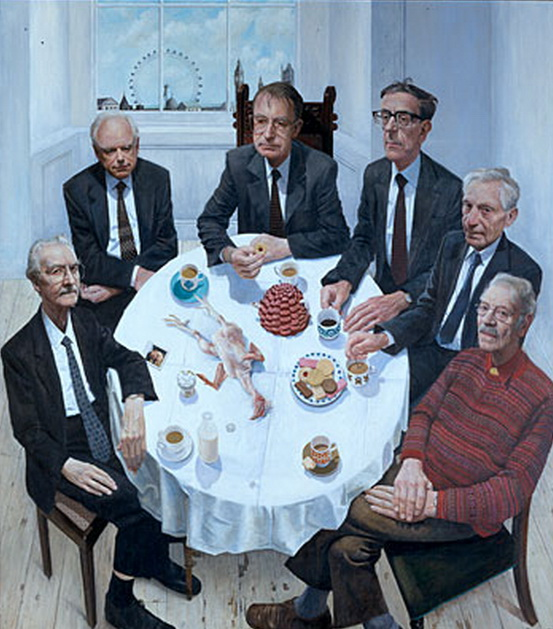
\includegraphics[height=\textheight]{stuartpearson}
\clearpage

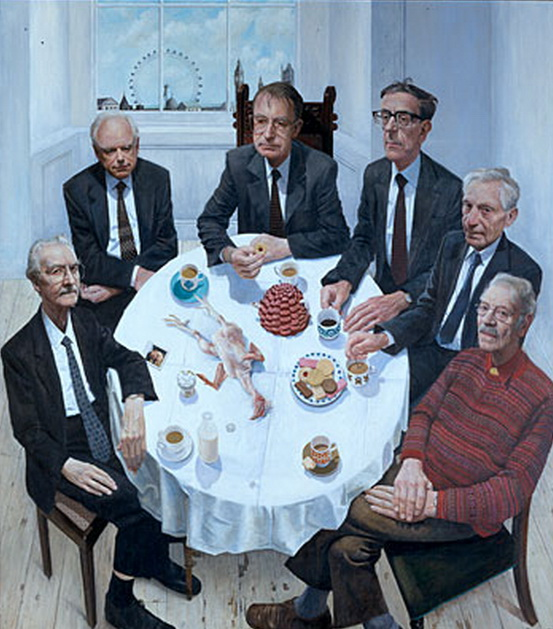
\includegraphics[height=\textheight]{stuartpearson}


\restoregeometry
\newpage \newpage
\def\printlayout{
\begin{tikzpicture}[scale=0.5]
\coordinate (pageX1) at (0,\paperheight);
\coordinate (text1) at (1in+\innermargin,\paperheight-1in-\headsep-\headheight);
% draw paper
\draw [color=red] (pageX1) rectangle ++(\paperwidth, -\paperheight);
% draw one inch around
\draw [color=blue] (1in, 0) -- ++(0, \paperheight);
\draw [color=blue] (0, \paperheight-1in) -- ++ (\paperwidth,0);
% draw textarea
\draw [color=green] (text1) rectangle ++ (\textwidth ,-\textheight);
% oddside margin
\draw [color=blue] (1in+\innermargin, \paperheight-1in-\headsep-\headheight) -- ++ (0,-\textheight);
% marginpar
\draw [color=blue] (1in+\innermargin+\textwidth+\marginparsep,\paperheight-1in-\headsep-\headheight ) rectangle ++(\marginparwidth,-\textheight);
\end{tikzpicture}

\printgeometryvalues}


\printlayout

\printlayout

\end{document} 